\documentclass[xetex]{beamer}

\mode<presentation> {
  \usetheme{Frankfurt}
  \setbeamercovered{transparent}
}

\usepackage{xunicode}
\usepackage{xltxtra}
\usepackage[czech]{babel}
\usepackage{palatino}
\usepackage{graphicx}
\usepackage{textpos}

%\usepackage{listings}
%\lstset{language=bash,
%        numbers=left,
%       numberstyle=\tiny,
%        showstringspaces=false,
%        aboveskip=-40pt,
%        frame=leftline
%        }

\title{Linux}

\author{Ondřej Profant}
\institute[Piráti]{Česká pirátská strana}
\date{\today}

\begin{document}

\begin{frame}
  \begin{textblock*}{0cm}(-1.2cm,-4.2cm)
  %
\includegraphics[scale=1.2]{images/intro.jpg}
  \end{textblock*}
\end{frame}

\begin{frame}
  \titlepage
\end{frame}

\begin{frame}
  \frametitle{Osnova}
  \tableofcontents
\end{frame}	


\section{GNU/LINUX}
\begin{frame}
	\frametitle{GNU/LINUX - úvod}

\end{frame}

\begin{frame}
	\frametitle{GNU/LINUX - rozšíření}

\end{frame}

\subsection{Distrubuce}
\begin{frame}
	\frametitle{Distribuce}
	\begin{itemize}
		\item Debian 
		\begin{itemize}
			\item Ubuntu
			\item Mint
			\item SteamOS
		\end{itemize}
		\item rpm
		\begin{itemize}
			\item Red Hat
			\item Fedora
		\end{itemize}
		\item Android
		\item Firefox OS
	\end{itemize}
\end{frame}

\subsection{Grafická prostředí}
\begin{frame}
	\frametitle{Grafická prostředí}
	\begin{itemize}
		\item KDE
		\item Gnome
		\item XFCE
		\item OpenBox
	\end{itemize}
\end{frame}


\begin{frame}
	\frametitle{Creative Commons}
	
	%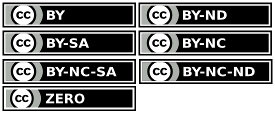
\includegraphics[scale=0.7]{images/cc-types.jpg}
\end{frame}

\subsection{RSS}
\begin{frame}
	\frametitle{RSS}

	Formát pro výměnu informací.

	\medskip

	Dnes sice velmi rozířen, ale zároveň zprzněn.

	\bigskip

%	
\includegraphics[scale=0.7]{images/rss.jpg}
\end{frame}

\section{Odpůrci svobody informací}
\begin{frame}
	\frametitle{Odpůrci svobody informací}
	\begin{enumerate}
		\item Ti kdo se informací bojí
		\item Ti kdo chtějí na informacích vydělávat
	\end{enumerate}

%	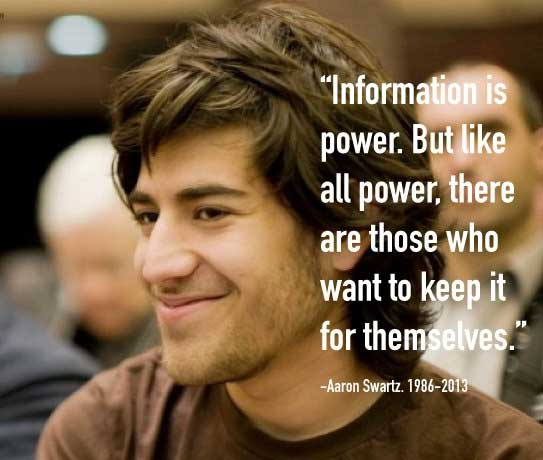
\includegraphics[scale=0.3]{images/information.jpg}
\end{frame}

\section{Příběh bojovníka}
\begin{frame}
	\frametitle{Příběh bojovníka - Aaron Swartz}
	Narozen 8. listopadu 1986

	\begin{itemize}
		\item ve čtrnácti letech se podílel na specifikaci RSS 1.0
		\item vytvořil webový framework web.py
		\item pracoval na tor2web, markdown, rozšíření HTTPS Everywhere pro Chrome
		\item stál u zrodu Creative commons
		\item spolupracoval na Open Library, Internet Archive, Demand Progress a Reddit
	\end{itemize}

\end{frame}

\begin{frame}
	\frametitle{JSTOR}
	Aaron stáhl v~kampusu MIT 4 000 000 vědeckých článků z JSTOR

	\bigskip

	Obviněn z porušení Computer Fraud and Abuse Act (CFAA).

	Kumulovaný trest: \$1 000 000, 35 let odnětí svobody.
\end{frame}

\begin{frame}
	%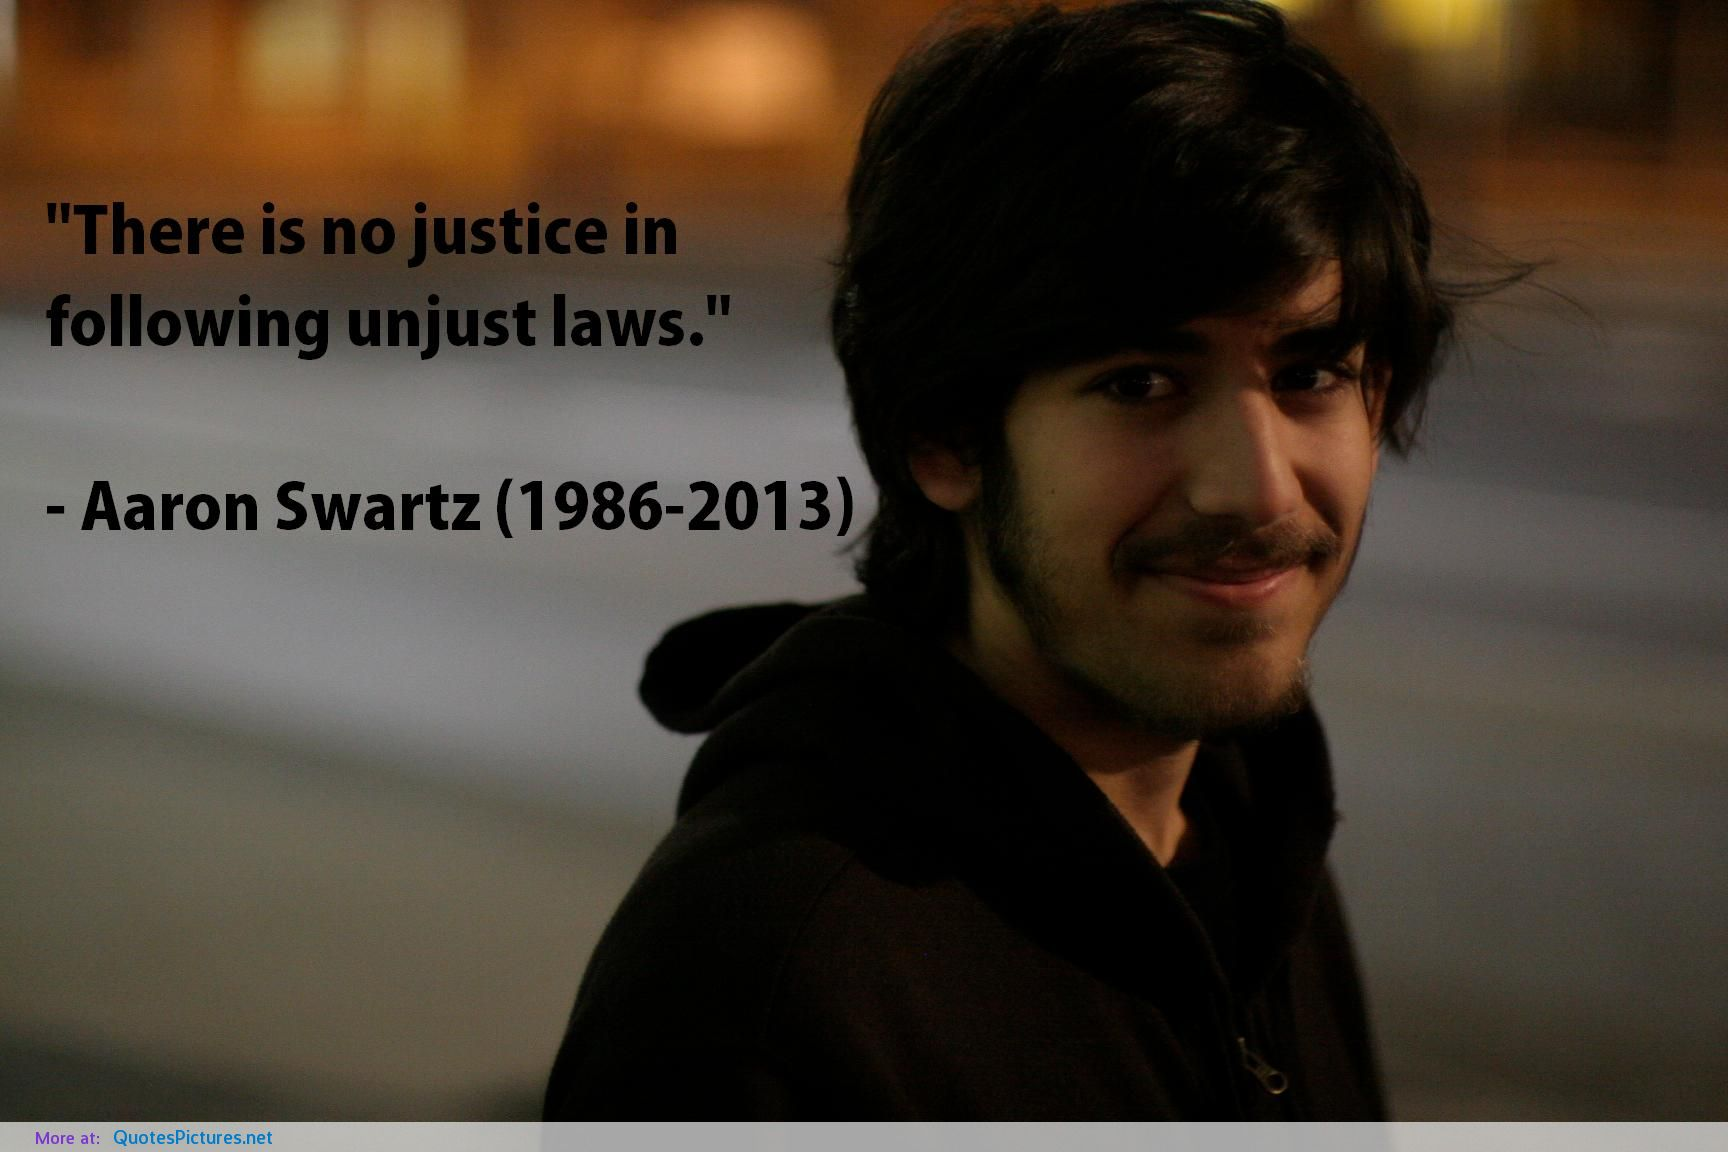
\includegraphics[scale=0.15]{images/no-justice.jpg}
\end{frame}

\section{Odkaz hrdiny}
\begin{frame}
	\frametitle{Odkaz hrdiny}
	\#pdftribute \url{http://pdftribute.net} \url{http://pdftribute.org}
\end{frame}

%	\url{http://en.wikipedia.org/wiki/Aaron_Swartz}\\
%	\url{http://www.rememberaaronsw.com}
%https://github.com/aaronsw
%https://forum.pirati.cz/post188796.html#p188796
%http://www.abclinuxu.cz/zpravicky/odesel-aaron-swartz-vyjimecny-hacker-a-aktivista

\begin{frame}

	Děkuji za pozornost.

	\bigskip
	
	Doplňující otázky?

	\bigskip

	\bigskip

	\scriptsize
	Copyleft Ondřej Profant, 2014. 
	Všechna práva vyhlazena. Sdílejte, upravujte a~nechte sdílet za stejných podmínek. 

	\bigskip

	Prezentace v~úplné formě\footnote{i se zdrojovými kódy} na:\\ 
	\url{https://www.github.com/kedrigern/prezentace-cs}.

	\bigskip

	Mail: ondrej.profant -at- pirati.cz 
\end{frame}

\end{document}
